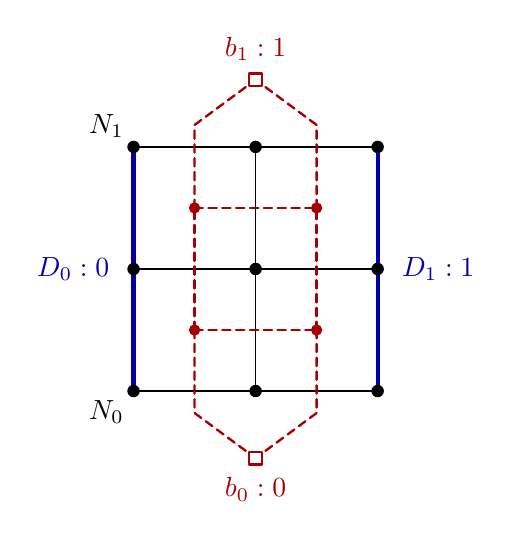
\begin{tikzpicture}[scale=1.55, line cap=round, line join=round,
    primal/.style={draw=black, line width=.65pt},
    prescribed/.style={draw=blue!65!black, line width=1.5pt},
    dual/.style={draw=red!65!black, densely dashed, line width=.85pt},
    face/.style={circle, fill=red!65!black, inner sep=1.45pt},
    wire/.style={rectangle, draw=red!65!black, fill=white,
                 line width=.9pt, inner sep=2.3pt}]
  \draw[primal] (0,0) grid (2,2);
  \draw[prescribed] (0,0)--(0,2);
  \draw[prescribed] (2,0)--(2,2);

  \draw[dual] (.5,.5)--(1.5,.5);
  \draw[dual] (.5,1.5)--(1.5,1.5);
  \draw[dual] (.5,.5)--(.5,1.5);
  \draw[dual] (1.5,.5)--(1.5,1.5);
  \draw[dual] (.5,.5)--(.5,-.18)--(1,-.55);
  \draw[dual] (1.5,.5)--(1.5,-.18)--(1,-.55);
  \draw[dual] (.5,1.5)--(.5,2.18)--(1,2.55);
  \draw[dual] (1.5,1.5)--(1.5,2.18)--(1,2.55);

  \foreach \x in {0,1,2}
    \foreach \y in {0,1,2}
      \fill[black] (\x,\y) circle (1.45pt);
  \foreach \x in {.5,1.5}
    \foreach \y in {.5,1.5}
      \node[face] at (\x,\y) {};
  \node[wire] at (1,-.55) {};
  \node[wire] at (1,2.55) {};

  \node[left, text=blue!65!black] at (-.12,1) {\(D_0:0\)};
  \node[right, text=blue!65!black] at (2.12,1) {\(D_1:1\)};
  \node[below left] at (0,0) {\(N_0\)};
  \node[above left] at (0,2) {\(N_1\)};
  \node[below, text=red!65!black] at (1,-.63) {\(b_0:0\)};
  \node[above, text=red!65!black] at (1,2.63) {\(b_1:1\)};
\end{tikzpicture}
